The interface subsystems are responsible for getting user input and translating it to the motion of the rover.

\subsection{User Interface}
This is the user interface, where users will be able to input which path-finding algorithm they want the rover to utilize, and control the motion of the rover.

\begin{figure}[h!]
	\centering
 	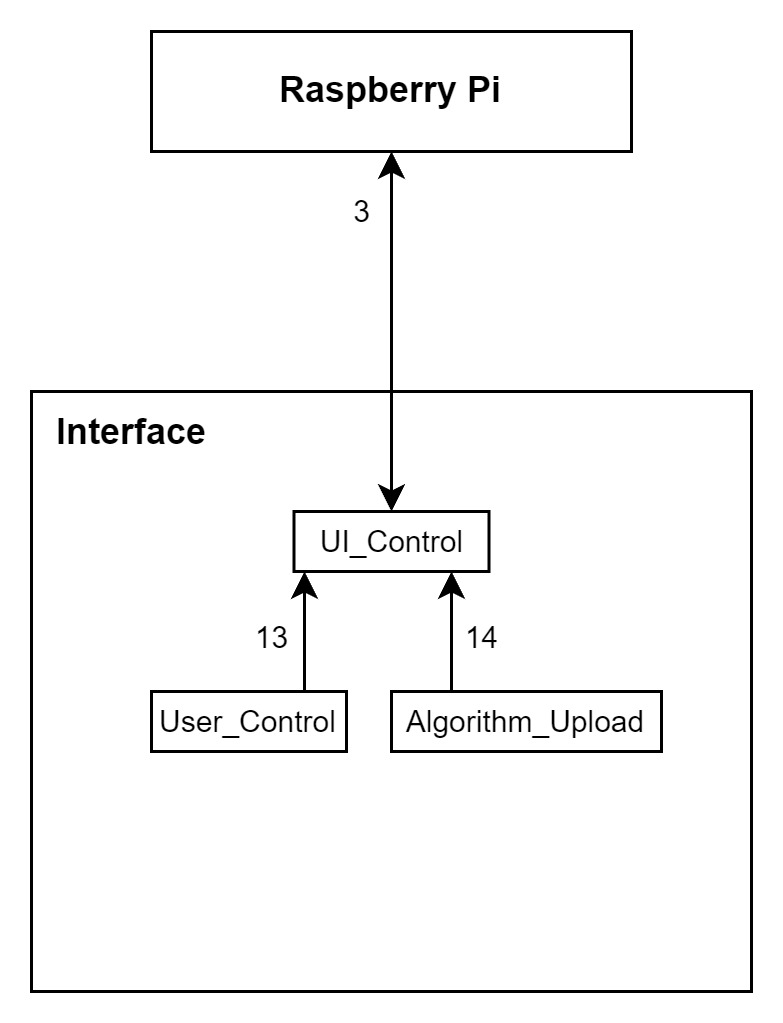
\includegraphics[width=0.45\textwidth]{images/interface/interface.jpg}
 \caption{Interface Subsystem} % Be sure to change the caption
\end{figure}

%%%%%%%%%%%%%%%%%%%%%%%%%%%%%%%%%%%%%%%%%%%%%%%%%%%%%%%%%%%%%%%%%%%%%%%%%%%%
%   Change the graphic here. Put your image in the 'images' folder
%   and update the name from 'images/test_image' to your image name

%\begin{figure}[h!]
	%\centering
 	%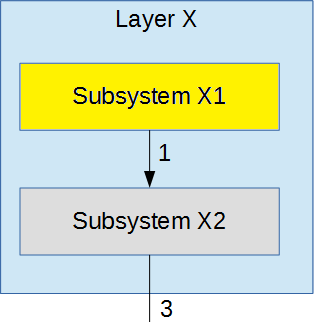
\includegraphics[width=0.60\textwidth]{images/subsystem}
 %\caption{Example subsystem description diagram} % Be sure to change the caption.
%\end{figure}


\subsubsection{Assumptions}
We are assuming that the user will be able to utilize the UI. We will be printing out specific instructions, and cover for any possible cases.

\subsubsection{Responsibilities}
It should be user-friendly and easy to use, so that users can simply run the program and send commands to the rover.

\subsubsection{Subsystem Interfaces}
%Each of the inputs and outputs for the subsystem are defined here. Create a table with an entry for each labelled interface that connects to this subsystem. For each entry, describe any incoming and outgoing data elements will pass through this interface.

\begin {table}[H]
\caption {Interface Subsystem} 
\begin{center}
    \begin{tabular}{ | p{1cm} | p{6cm} | p{3cm} | p{3cm} |}
    \hline
    ID & Description & Inputs & Outputs \\ \hline
    \#3 & UI & \pbox{3cm}{N/A} & \pbox{3cm}{Screen}  \\ \hline
    \#13 & User Control & \pbox{3cm}{Speed \\ Direction} & \pbox{3cm}{Motion}  \\ \hline
    \#14 & Algorithm Upload & \pbox{3cm}{Algorithm Name} & \pbox{3cm}{Path-finding}  \\ \hline
    
    \end{tabular}
\end{center}
\end{table}

%\subsection{Subsystem 2}
%Repeat for each subsystem

%\subsection{Subsystem 3}
%Repeat for each subsystem

